% Created by tikzDevice version 0.12.3.1 on 2021-02-08 17:04:18
% !TEX encoding = UTF-8 Unicode
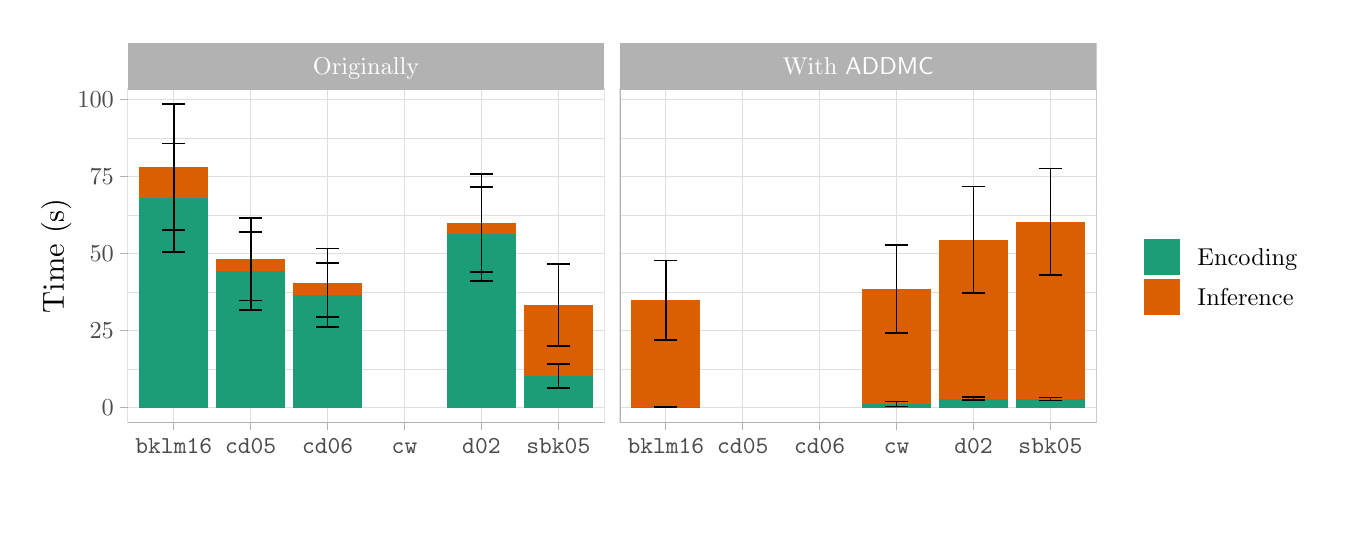
\begin{tikzpicture}[x=1pt,y=1pt]
\definecolor{fillColor}{RGB}{255,255,255}
\path[use as bounding box,fill=fillColor,fill opacity=0.00] (0,0) rectangle (469.75,173.45);
\begin{scope}
\path[clip] (  0.00,  0.00) rectangle (469.75,173.45);
\definecolor{drawColor}{RGB}{255,255,255}
\definecolor{fillColor}{RGB}{255,255,255}

\path[draw=drawColor,line width= 0.6pt,line join=round,line cap=round,fill=fillColor] (  0.00,  0.00) rectangle (469.75,173.45);
\end{scope}
\begin{scope}
\path[clip] ( 36.11, 30.69) rectangle (208.43,151.38);
\definecolor{fillColor}{RGB}{255,255,255}

\path[fill=fillColor] ( 36.11, 30.69) rectangle (208.43,151.38);
\definecolor{drawColor}{gray}{0.87}

\path[draw=drawColor,line width= 0.1pt,line join=round] ( 36.11, 50.08) --
	(208.43, 50.08);

\path[draw=drawColor,line width= 0.1pt,line join=round] ( 36.11, 77.91) --
	(208.43, 77.91);

\path[draw=drawColor,line width= 0.1pt,line join=round] ( 36.11,105.73) --
	(208.43,105.73);

\path[draw=drawColor,line width= 0.1pt,line join=round] ( 36.11,133.56) --
	(208.43,133.56);

\path[draw=drawColor,line width= 0.3pt,line join=round] ( 36.11, 36.17) --
	(208.43, 36.17);

\path[draw=drawColor,line width= 0.3pt,line join=round] ( 36.11, 64.00) --
	(208.43, 64.00);

\path[draw=drawColor,line width= 0.3pt,line join=round] ( 36.11, 91.82) --
	(208.43, 91.82);

\path[draw=drawColor,line width= 0.3pt,line join=round] ( 36.11,119.64) --
	(208.43,119.64);

\path[draw=drawColor,line width= 0.3pt,line join=round] ( 36.11,147.47) --
	(208.43,147.47);

\path[draw=drawColor,line width= 0.3pt,line join=round] ( 52.79, 30.69) --
	( 52.79,151.38);

\path[draw=drawColor,line width= 0.3pt,line join=round] ( 80.58, 30.69) --
	( 80.58,151.38);

\path[draw=drawColor,line width= 0.3pt,line join=round] (108.37, 30.69) --
	(108.37,151.38);

\path[draw=drawColor,line width= 0.3pt,line join=round] (136.17, 30.69) --
	(136.17,151.38);

\path[draw=drawColor,line width= 0.3pt,line join=round] (163.96, 30.69) --
	(163.96,151.38);

\path[draw=drawColor,line width= 0.3pt,line join=round] (191.76, 30.69) --
	(191.76,151.38);
\definecolor{fillColor}{RGB}{27,158,119}

\path[fill=fillColor] ( 40.28, 36.17) rectangle ( 65.29,111.99);
\definecolor{fillColor}{RGB}{217,95,2}

\path[fill=fillColor] ( 40.28,111.99) rectangle ( 65.29,123.08);
\definecolor{fillColor}{RGB}{27,158,119}

\path[fill=fillColor] ( 68.07, 36.17) rectangle ( 93.09, 85.55);
\definecolor{fillColor}{RGB}{217,95,2}

\path[fill=fillColor] ( 68.07, 85.55) rectangle ( 93.09, 89.74);
\definecolor{fillColor}{RGB}{27,158,119}

\path[fill=fillColor] ( 95.87, 36.17) rectangle (120.88, 76.88);
\definecolor{fillColor}{RGB}{217,95,2}

\path[fill=fillColor] ( 95.87, 76.88) rectangle (120.88, 81.34);
\definecolor{fillColor}{RGB}{27,158,119}

\path[fill=fillColor] (151.46, 36.17) rectangle (176.47, 98.96);
\definecolor{fillColor}{RGB}{217,95,2}

\path[fill=fillColor] (151.46, 98.96) rectangle (176.47,102.91);
\definecolor{fillColor}{RGB}{27,158,119}

\path[fill=fillColor] (179.25, 36.17) rectangle (204.26, 47.56);
\definecolor{fillColor}{RGB}{217,95,2}

\path[fill=fillColor] (179.25, 47.56) rectangle (204.26, 73.20);
\definecolor{drawColor}{RGB}{0,0,0}

\path[draw=drawColor,line width= 0.6pt,line join=round] ( 48.62,131.57) --
	( 56.96,131.57);

\path[draw=drawColor,line width= 0.6pt,line join=round] ( 52.79,131.57) --
	( 52.79, 92.41);

\path[draw=drawColor,line width= 0.6pt,line join=round] ( 48.62, 92.41) --
	( 56.96, 92.41);

\path[draw=drawColor,line width= 0.6pt,line join=round] ( 48.62,145.89) --
	( 56.96,145.89);

\path[draw=drawColor,line width= 0.6pt,line join=round] ( 52.79,145.89) --
	( 52.79,100.26);

\path[draw=drawColor,line width= 0.6pt,line join=round] ( 48.62,100.26) --
	( 56.96,100.26);

\path[draw=drawColor,line width= 0.6pt,line join=round] ( 76.41, 99.71) --
	( 84.75, 99.71);

\path[draw=drawColor,line width= 0.6pt,line join=round] ( 80.58, 99.71) --
	( 80.58, 71.38);

\path[draw=drawColor,line width= 0.6pt,line join=round] ( 76.41, 71.38) --
	( 84.75, 71.38);

\path[draw=drawColor,line width= 0.6pt,line join=round] ( 76.41,104.66) --
	( 84.75,104.66);

\path[draw=drawColor,line width= 0.6pt,line join=round] ( 80.58,104.66) --
	( 80.58, 74.82);

\path[draw=drawColor,line width= 0.6pt,line join=round] ( 76.41, 74.82) --
	( 84.75, 74.82);

\path[draw=drawColor,line width= 0.6pt,line join=round] (104.21, 88.40) --
	(112.54, 88.40);

\path[draw=drawColor,line width= 0.6pt,line join=round] (108.37, 88.40) --
	(108.37, 65.36);

\path[draw=drawColor,line width= 0.6pt,line join=round] (104.21, 65.36) --
	(112.54, 65.36);

\path[draw=drawColor,line width= 0.6pt,line join=round] (104.21, 93.67) --
	(112.54, 93.67);

\path[draw=drawColor,line width= 0.6pt,line join=round] (108.37, 93.67) --
	(108.37, 69.01);

\path[draw=drawColor,line width= 0.6pt,line join=round] (104.21, 69.01) --
	(112.54, 69.01);

\path[draw=drawColor,line width= 0.6pt,line join=round] (159.79,115.90) --
	(168.13,115.90);

\path[draw=drawColor,line width= 0.6pt,line join=round] (163.96,115.90) --
	(163.96, 82.02);

\path[draw=drawColor,line width= 0.6pt,line join=round] (159.79, 82.02) --
	(168.13, 82.02);

\path[draw=drawColor,line width= 0.6pt,line join=round] (159.79,120.62) --
	(168.13,120.62);

\path[draw=drawColor,line width= 0.6pt,line join=round] (163.96,120.62) --
	(163.96, 85.20);

\path[draw=drawColor,line width= 0.6pt,line join=round] (159.79, 85.20) --
	(168.13, 85.20);

\path[draw=drawColor,line width= 0.6pt,line join=round] (187.59, 51.93) --
	(195.93, 51.93);

\path[draw=drawColor,line width= 0.6pt,line join=round] (191.76, 51.93) --
	(191.76, 43.18);

\path[draw=drawColor,line width= 0.6pt,line join=round] (187.59, 43.18) --
	(195.93, 43.18);

\path[draw=drawColor,line width= 0.6pt,line join=round] (187.59, 88.00) --
	(195.93, 88.00);

\path[draw=drawColor,line width= 0.6pt,line join=round] (191.76, 88.00) --
	(191.76, 58.41);

\path[draw=drawColor,line width= 0.6pt,line join=round] (187.59, 58.41) --
	(195.93, 58.41);
\definecolor{drawColor}{gray}{0.70}

\path[draw=drawColor,line width= 0.6pt,line join=round,line cap=round] ( 36.11, 30.69) rectangle (208.43,151.38);
\end{scope}
\begin{scope}
\path[clip] (213.93, 30.69) rectangle (386.25,151.38);
\definecolor{fillColor}{RGB}{255,255,255}

\path[fill=fillColor] (213.93, 30.69) rectangle (386.25,151.38);
\definecolor{drawColor}{gray}{0.87}

\path[draw=drawColor,line width= 0.1pt,line join=round] (213.93, 50.08) --
	(386.25, 50.08);

\path[draw=drawColor,line width= 0.1pt,line join=round] (213.93, 77.91) --
	(386.25, 77.91);

\path[draw=drawColor,line width= 0.1pt,line join=round] (213.93,105.73) --
	(386.25,105.73);

\path[draw=drawColor,line width= 0.1pt,line join=round] (213.93,133.56) --
	(386.25,133.56);

\path[draw=drawColor,line width= 0.3pt,line join=round] (213.93, 36.17) --
	(386.25, 36.17);

\path[draw=drawColor,line width= 0.3pt,line join=round] (213.93, 64.00) --
	(386.25, 64.00);

\path[draw=drawColor,line width= 0.3pt,line join=round] (213.93, 91.82) --
	(386.25, 91.82);

\path[draw=drawColor,line width= 0.3pt,line join=round] (213.93,119.64) --
	(386.25,119.64);

\path[draw=drawColor,line width= 0.3pt,line join=round] (213.93,147.47) --
	(386.25,147.47);

\path[draw=drawColor,line width= 0.3pt,line join=round] (230.61, 30.69) --
	(230.61,151.38);

\path[draw=drawColor,line width= 0.3pt,line join=round] (258.40, 30.69) --
	(258.40,151.38);

\path[draw=drawColor,line width= 0.3pt,line join=round] (286.20, 30.69) --
	(286.20,151.38);

\path[draw=drawColor,line width= 0.3pt,line join=round] (313.99, 30.69) --
	(313.99,151.38);

\path[draw=drawColor,line width= 0.3pt,line join=round] (341.78, 30.69) --
	(341.78,151.38);

\path[draw=drawColor,line width= 0.3pt,line join=round] (369.58, 30.69) --
	(369.58,151.38);
\definecolor{fillColor}{RGB}{27,158,119}

\path[fill=fillColor] (218.10, 36.17) rectangle (243.12, 36.39);
\definecolor{fillColor}{RGB}{217,95,2}

\path[fill=fillColor] (218.10, 36.39) rectangle (243.12, 74.95);
\definecolor{fillColor}{RGB}{27,158,119}

\path[fill=fillColor] (301.48, 36.17) rectangle (326.50, 37.47);
\definecolor{fillColor}{RGB}{217,95,2}

\path[fill=fillColor] (301.48, 37.47) rectangle (326.50, 78.97);
\definecolor{fillColor}{RGB}{27,158,119}

\path[fill=fillColor] (329.28, 36.17) rectangle (354.29, 39.40);
\definecolor{fillColor}{RGB}{217,95,2}

\path[fill=fillColor] (329.28, 39.40) rectangle (354.29, 96.79);
\definecolor{fillColor}{RGB}{27,158,119}

\path[fill=fillColor] (357.07, 36.17) rectangle (382.08, 39.31);
\definecolor{fillColor}{RGB}{217,95,2}

\path[fill=fillColor] (357.07, 39.31) rectangle (382.08,103.33);
\definecolor{drawColor}{RGB}{0,0,0}

\path[draw=drawColor,line width= 0.6pt,line join=round] (226.44, 36.50) --
	(234.78, 36.50);

\path[draw=drawColor,line width= 0.6pt,line join=round] (230.61, 36.50) --
	(230.61, 36.29);

\path[draw=drawColor,line width= 0.6pt,line join=round] (226.44, 36.29) --
	(234.78, 36.29);

\path[draw=drawColor,line width= 0.6pt,line join=round] (226.44, 89.26) --
	(234.78, 89.26);

\path[draw=drawColor,line width= 0.6pt,line join=round] (230.61, 89.26) --
	(230.61, 60.63);

\path[draw=drawColor,line width= 0.6pt,line join=round] (226.44, 60.63) --
	(234.78, 60.63);

\path[draw=drawColor,line width= 0.6pt,line join=round] (309.82, 38.33) --
	(318.16, 38.33);

\path[draw=drawColor,line width= 0.6pt,line join=round] (313.99, 38.33) --
	(313.99, 36.60);

\path[draw=drawColor,line width= 0.6pt,line join=round] (309.82, 36.60) --
	(318.16, 36.60);

\path[draw=drawColor,line width= 0.6pt,line join=round] (309.82, 94.93) --
	(318.16, 94.93);

\path[draw=drawColor,line width= 0.6pt,line join=round] (313.99, 94.93) --
	(313.99, 63.01);

\path[draw=drawColor,line width= 0.6pt,line join=round] (309.82, 63.01) --
	(318.16, 63.01);

\path[draw=drawColor,line width= 0.6pt,line join=round] (337.61, 39.96) --
	(345.95, 39.96);

\path[draw=drawColor,line width= 0.6pt,line join=round] (341.78, 39.96) --
	(341.78, 38.83);

\path[draw=drawColor,line width= 0.6pt,line join=round] (337.61, 38.83) --
	(345.95, 38.83);

\path[draw=drawColor,line width= 0.6pt,line join=round] (337.61,116.01) --
	(345.95,116.01);

\path[draw=drawColor,line width= 0.6pt,line join=round] (341.78,116.01) --
	(341.78, 77.57);

\path[draw=drawColor,line width= 0.6pt,line join=round] (337.61, 77.57) --
	(345.95, 77.57);

\path[draw=drawColor,line width= 0.6pt,line join=round] (365.41, 39.85) --
	(373.75, 39.85);

\path[draw=drawColor,line width= 0.6pt,line join=round] (369.58, 39.85) --
	(369.58, 38.76);

\path[draw=drawColor,line width= 0.6pt,line join=round] (365.41, 38.76) --
	(373.75, 38.76);

\path[draw=drawColor,line width= 0.6pt,line join=round] (365.41,122.50) --
	(373.75,122.50);

\path[draw=drawColor,line width= 0.6pt,line join=round] (369.58,122.50) --
	(369.58, 84.17);

\path[draw=drawColor,line width= 0.6pt,line join=round] (365.41, 84.17) --
	(373.75, 84.17);
\definecolor{drawColor}{gray}{0.70}

\path[draw=drawColor,line width= 0.6pt,line join=round,line cap=round] (213.93, 30.69) rectangle (386.25,151.38);
\end{scope}
\begin{scope}
\path[clip] ( 36.11,151.38) rectangle (208.43,167.95);
\definecolor{fillColor}{gray}{0.70}

\path[fill=fillColor] ( 36.11,151.38) rectangle (208.43,167.95);
\definecolor{drawColor}{RGB}{255,255,255}

\node[text=drawColor,anchor=base,inner sep=0pt, outer sep=0pt, scale=  0.88] at (122.27,156.63) {Originally};
\end{scope}
\begin{scope}
\path[clip] (213.93,151.38) rectangle (386.25,167.95);
\definecolor{fillColor}{gray}{0.70}

\path[fill=fillColor] (213.93,151.38) rectangle (386.25,167.95);
\definecolor{drawColor}{RGB}{255,255,255}

\node[text=drawColor,anchor=base,inner sep=0pt, outer sep=0pt, scale=  0.88] at (300.09,156.63) {With \textsf{ADDMC}};
\end{scope}
\begin{scope}
\path[clip] (  0.00,  0.00) rectangle (469.75,173.45);
\definecolor{drawColor}{gray}{0.70}

\path[draw=drawColor,line width= 0.3pt,line join=round] ( 52.79, 27.94) --
	( 52.79, 30.69);

\path[draw=drawColor,line width= 0.3pt,line join=round] ( 80.58, 27.94) --
	( 80.58, 30.69);

\path[draw=drawColor,line width= 0.3pt,line join=round] (108.37, 27.94) --
	(108.37, 30.69);

\path[draw=drawColor,line width= 0.3pt,line join=round] (136.17, 27.94) --
	(136.17, 30.69);

\path[draw=drawColor,line width= 0.3pt,line join=round] (163.96, 27.94) --
	(163.96, 30.69);

\path[draw=drawColor,line width= 0.3pt,line join=round] (191.76, 27.94) --
	(191.76, 30.69);
\end{scope}
\begin{scope}
\path[clip] (  0.00,  0.00) rectangle (469.75,173.45);
\definecolor{drawColor}{gray}{0.30}

\node[text=drawColor,anchor=base,inner sep=0pt, outer sep=0pt, scale=  0.88] at ( 52.79, 19.68) {\texttt{bklm16}};

\node[text=drawColor,anchor=base,inner sep=0pt, outer sep=0pt, scale=  0.88] at ( 80.58, 19.68) {\texttt{cd05}};

\node[text=drawColor,anchor=base,inner sep=0pt, outer sep=0pt, scale=  0.88] at (108.37, 19.68) {\texttt{cd06}};

\node[text=drawColor,anchor=base,inner sep=0pt, outer sep=0pt, scale=  0.88] at (136.17, 19.68) {\texttt{cw}};

\node[text=drawColor,anchor=base,inner sep=0pt, outer sep=0pt, scale=  0.88] at (163.96, 19.68) {\texttt{d02}};

\node[text=drawColor,anchor=base,inner sep=0pt, outer sep=0pt, scale=  0.88] at (191.76, 19.68) {\texttt{sbk05}};
\end{scope}
\begin{scope}
\path[clip] (  0.00,  0.00) rectangle (469.75,173.45);
\definecolor{drawColor}{gray}{0.70}

\path[draw=drawColor,line width= 0.3pt,line join=round] (230.61, 27.94) --
	(230.61, 30.69);

\path[draw=drawColor,line width= 0.3pt,line join=round] (258.40, 27.94) --
	(258.40, 30.69);

\path[draw=drawColor,line width= 0.3pt,line join=round] (286.20, 27.94) --
	(286.20, 30.69);

\path[draw=drawColor,line width= 0.3pt,line join=round] (313.99, 27.94) --
	(313.99, 30.69);

\path[draw=drawColor,line width= 0.3pt,line join=round] (341.78, 27.94) --
	(341.78, 30.69);

\path[draw=drawColor,line width= 0.3pt,line join=round] (369.58, 27.94) --
	(369.58, 30.69);
\end{scope}
\begin{scope}
\path[clip] (  0.00,  0.00) rectangle (469.75,173.45);
\definecolor{drawColor}{gray}{0.30}

\node[text=drawColor,anchor=base,inner sep=0pt, outer sep=0pt, scale=  0.88] at (230.61, 19.68) {\texttt{bklm16}};

\node[text=drawColor,anchor=base,inner sep=0pt, outer sep=0pt, scale=  0.88] at (258.40, 19.68) {\texttt{cd05}};

\node[text=drawColor,anchor=base,inner sep=0pt, outer sep=0pt, scale=  0.88] at (286.20, 19.68) {\texttt{cd06}};

\node[text=drawColor,anchor=base,inner sep=0pt, outer sep=0pt, scale=  0.88] at (313.99, 19.68) {\texttt{cw}};

\node[text=drawColor,anchor=base,inner sep=0pt, outer sep=0pt, scale=  0.88] at (341.78, 19.68) {\texttt{d02}};

\node[text=drawColor,anchor=base,inner sep=0pt, outer sep=0pt, scale=  0.88] at (369.58, 19.68) {\texttt{sbk05}};
\end{scope}
\begin{scope}
\path[clip] (  0.00,  0.00) rectangle (469.75,173.45);
\definecolor{drawColor}{gray}{0.30}

\node[text=drawColor,anchor=base east,inner sep=0pt, outer sep=0pt, scale=  0.88] at ( 31.16, 33.14) {0};

\node[text=drawColor,anchor=base east,inner sep=0pt, outer sep=0pt, scale=  0.88] at ( 31.16, 60.97) {25};

\node[text=drawColor,anchor=base east,inner sep=0pt, outer sep=0pt, scale=  0.88] at ( 31.16, 88.79) {50};

\node[text=drawColor,anchor=base east,inner sep=0pt, outer sep=0pt, scale=  0.88] at ( 31.16,116.61) {75};

\node[text=drawColor,anchor=base east,inner sep=0pt, outer sep=0pt, scale=  0.88] at ( 31.16,144.44) {100};
\end{scope}
\begin{scope}
\path[clip] (  0.00,  0.00) rectangle (469.75,173.45);
\definecolor{drawColor}{gray}{0.70}

\path[draw=drawColor,line width= 0.3pt,line join=round] ( 33.36, 36.17) --
	( 36.11, 36.17);

\path[draw=drawColor,line width= 0.3pt,line join=round] ( 33.36, 64.00) --
	( 36.11, 64.00);

\path[draw=drawColor,line width= 0.3pt,line join=round] ( 33.36, 91.82) --
	( 36.11, 91.82);

\path[draw=drawColor,line width= 0.3pt,line join=round] ( 33.36,119.64) --
	( 36.11,119.64);

\path[draw=drawColor,line width= 0.3pt,line join=round] ( 33.36,147.47) --
	( 36.11,147.47);
\end{scope}
\begin{scope}
\path[clip] (  0.00,  0.00) rectangle (469.75,173.45);
\definecolor{drawColor}{RGB}{0,0,0}

\node[text=drawColor,rotate= 90.00,anchor=base,inner sep=0pt, outer sep=0pt, scale=  1.10] at ( 13.08, 91.03) {Time (s)};
\end{scope}
\begin{scope}
\path[clip] (  0.00,  0.00) rectangle (469.75,173.45);
\definecolor{fillColor}{RGB}{255,255,255}

\path[fill=fillColor] (397.25, 63.47) rectangle (464.25,118.59);
\end{scope}
\begin{scope}
\path[clip] (  0.00,  0.00) rectangle (469.75,173.45);
\definecolor{fillColor}{RGB}{255,255,255}

\path[fill=fillColor] (402.75, 83.42) rectangle (417.21, 97.88);
\end{scope}
\begin{scope}
\path[clip] (  0.00,  0.00) rectangle (469.75,173.45);
\definecolor{fillColor}{RGB}{27,158,119}

\path[fill=fillColor] (403.47, 84.14) rectangle (416.50, 97.17);
\end{scope}
\begin{scope}
\path[clip] (  0.00,  0.00) rectangle (469.75,173.45);
\definecolor{fillColor}{RGB}{255,255,255}

\path[fill=fillColor] (402.75, 68.97) rectangle (417.21, 83.42);
\end{scope}
\begin{scope}
\path[clip] (  0.00,  0.00) rectangle (469.75,173.45);
\definecolor{fillColor}{RGB}{217,95,2}

\path[fill=fillColor] (403.47, 69.68) rectangle (416.50, 82.71);
\end{scope}
\begin{scope}
\path[clip] (  0.00,  0.00) rectangle (469.75,173.45);
\definecolor{drawColor}{RGB}{0,0,0}

\node[text=drawColor,anchor=base west,inner sep=0pt, outer sep=0pt, scale=  0.88] at (422.71, 87.62) {Encoding};
\end{scope}
\begin{scope}
\path[clip] (  0.00,  0.00) rectangle (469.75,173.45);
\definecolor{drawColor}{RGB}{0,0,0}

\node[text=drawColor,anchor=base west,inner sep=0pt, outer sep=0pt, scale=  0.88] at (422.71, 73.17) {Inference};
\end{scope}
\end{tikzpicture}
